%%% LaTeX Template: Article/Thesis/etc. with colored headings and special fonts
%%%
%%% Source: http://www.howtotex.com/
%%% Feel free to distribute this template, but please keep to referal to http://www.howtotex.com/ here.
%%% February 2011
%%%
%%% Modified January 2016 by CDM

%%%  Preamble
\documentclass[11pt,letterpaper]{article}
\usepackage[margin=1.0in]{geometry}
\usepackage[T1]{fontenc}
\usepackage[bitstream-charter]{mathdesign}
\usepackage[latin1]{inputenc}					
\usepackage{amsmath}						
\usepackage{xcolor}
\usepackage{cite}
\usepackage{hyphenat}
\usepackage{graphicx}
\usepackage{float}
\usepackage{subfigure}
\usepackage{sectsty}
\usepackage[compact]{titlesec} 
\usepackage[tablegrid]{vhistory}
\usepackage{pbox}
\allsectionsfont{\color{accentcolor}\scshape\selectfont}

%%% Definitions
\definecolor{accentcolor}{rgb}{0.0,0.0,0.5} 
\newcommand{\teamname}{3.14159}
\newcommand{\productname}{Traffic Pi}
\newcommand{\coursename}{CSE 4316: Senior Design I}
\newcommand{\semester}{Fall 2018}
\newcommand{\docname}{Architectural Design Specification}
\newcommand{\department}{Department of Computer Science \& Engineering}
\newcommand{\university}{The University of Texas at Arlington}
\newcommand{\authors}{Jacob Devasier \\ Ethan Duff \\ Seth Tisbi \\ Kevin Tiller \\ Miguel Fraire}

%%% Headers and footers
\usepackage{fancyhdr}
	\pagestyle{fancy}						% Enabling the custom headers/footers
\usepackage{lastpage}	
	% Header (empty)
	\lhead{}
	\chead{}
	\rhead{}
	% Footer
	\lfoot{\footnotesize \teamname \ - \semester}
	\cfoot{}
	\rfoot{\footnotesize page \thepage\ of \pageref{LastPage}}	% "Page 1 of 2"
	\renewcommand{\headrulewidth}{0.0pt}
	\renewcommand{\footrulewidth}{0.4pt}

%%% Change the abstract environment
\usepackage[runin]{abstract}			% runin option for a run-in title
%\setlength\absleftindent{30pt}			% left margin
%\setlength\absrightindent{30pt}		% right margin
\abslabeldelim{\quad}	
\setlength{\abstitleskip}{-10pt}
\renewcommand{\abstractname}{}
\renewcommand{\abstracttextfont}{\color{accentcolor} \small \slshape}	% slanted text

%%% Start of the document
\begin{document}

%%% Cover sheet
{\centering \huge \color{accentcolor} \sc \textbf{\department \\ \university} \par}
\vspace{1 in}
{\centering \huge \color{accentcolor} \sc \textbf{\docname \\ \coursename \\ \semester} \par}
\vspace{0.5 in}
\begin{figure}[h!]
	\centering
   	
\includegraphics[width=0.45\textwidth]{images/traffic_light}
\end{figure}
\vspace{0.5 in}
{\centering \huge \color{accentcolor} \sc \textbf{\teamname \\ \productname} \par}
\vspace{0.5 in}
{\centering \large \sc \textbf{\authors} \par}
\newpage


%\vspace{1 in}
%\centerline{January 13th, 2012}
%\newpage

%%% Revision History
\begin{versionhistory}
  	\vhEntry{0.1}{10.01.2018}{GH}{document creation}
  	\vhEntry{0.2}{10.05.2018}{AT|GH}{complete draft}
  	\vhEntry{0.3}{10.12.2018}{AT|GH}{release candidate 1}
  	\vhEntry{1.0}{10.20.2018}{AT|GH|CB}{official release}
  	\vhEntry{1.1}{10.31.2018}{AL}{added design review requests}
  	\vhEntry{1.2}{12.03.2018}{JD|ED|MF|KT|ST}{error correction}
\end{versionhistory}
\newpage

%%% Table of contents
\setcounter{tocdepth}{2}
\tableofcontents
\newpage

%%% List of figures and tables (optional)
\listoffigures
\listoftables
\newpage

%%% Document sections
\section{Introduction}
The system as a whole is designed to record passing traffic and run an analysis on collected data in order to produce a coherent collection of cars breaking the speed limit to determine if further civil actions need to be taken to increase the safety of the road.  The system requires a mounted case that will contain a raspberry pi computer attached to multiple cameras.  These cameras will record the traffic of a nearby road, saving video files of sections when cars have passed.  This information will be processed on a host computer once the device has been taken in and connected.  An application will analyze the data and provide results back to the user.
\newpage
\section{System Overview}
The architecture revolves primarily around the raspberry pi computer itself.  The interface of the raspberry pi will communicate with all other major systems sending commands and receiving data.  The first major system to communicate with is the vision system.  This system is responsible for the cameras and has two that are part of it: the IR camera, and the 3D camera.  Both will connect to the PI's interface in order to transmit visual data.  This data will be redirected by the interface to the Pre-processing unit which will determine what raw film data is worth keeping and what is not by a factor of cars in the streets.  Data kept is placed into storage which the interface can then pull out again.  It is powered by a socket connected to the power system, an outlet inside the users home.  The case system has a cooling unit which prevents the PI from overheating through a ventilation shaft.  This fan draws power from the PI via its interface.  When the PI is connected to the user's computer via Ethernet, it will automatically run its application on their computer.  This application receives transferred data from the PI's storage and processes it, splitting meta data into a database and film data into local storage.  All of this data will be accessible to the user via a graphic user interface.

\begin{figure}[h!]
	\centering
 	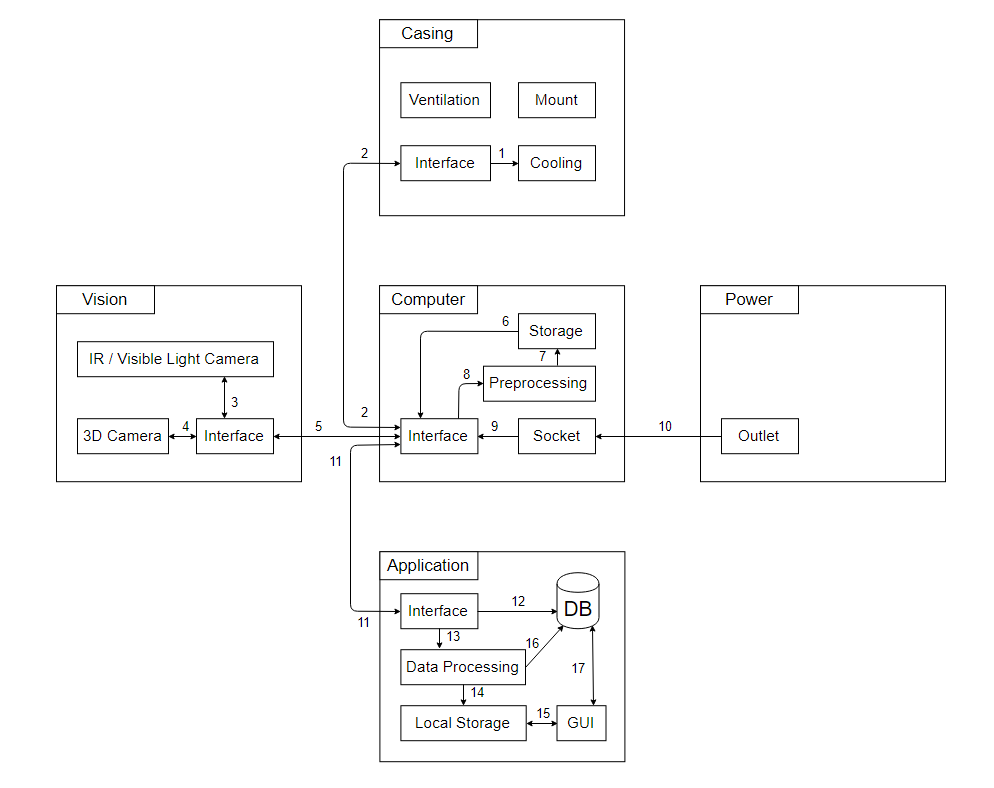
\includegraphics[width=0.60\textwidth]{images/ADS.png}
 \caption{A simple architectural layer diagram}
\end{figure}

\subsection{Layer Computer Description}
The main purpose of the computer layer is to the central source of communication and serve as the collector and organizer of data received from the vision layer. Maintaining power granted by the power layer and distribute to the cooling system, cameras, and itself to function as desired. Allowing to request proper cooling from the case layer to maintain functionality of the Traffic Pi without worrying about unstable temperature both generated from internal and environmental. The computer layer will take in raw data from the vision layer, such as footage (frames), distance, and lighting, after detecting cars passing by. Pre-processing will take in effect, time stamping frames and formatting data, then direct to the storage for later use by the application layer.

\subsection{Layer Vision Description}
The vision layer comprises of the physical cameras, IR / visible light and 3D cameras, that views the road and transmit the footage data to the Traffic Pi's pre-processing and stored for later. The IR / visible light camera would be able to view the road and passing vehicles in both day and night settings. The 3D camera will be able to measure the distance of the passing vehicles from the camera in every passing frames. While collecting data, until function completion is met, the footage / frames and distance will to send to the computer layer.

\subsection{Layer Application Description}
The main purpose of the application layer is to handle the actual processing of the raw video on the users local machine coming from the computer layer. During the video processing, bounding boxes will be placed around every appropriate vehicle and speed will be measured and recorded. The resulting data will be stored on a local database. Meanwhile, the resulting video will be stored on the users local storage. This layer provides the user with a graphical user interface in order to interact with the system. Using the GUI, the user will be able to view the analyzed video and will have the option be presented with a dashboard fitted with the visual representation of the analytics regarding the traffic study. The user will also have the option of a quick guide and options to download the file of data.

\subsection{Layer Case Description}
The case layer is designed to house every component in a self contained physical structure. The case is designed such that the heat generated from the Raspberry Pi, IR camera, and 3D camera will be able to dissipate quickly away from the system. This ventilation works in conjunction with the cooling subsystem. The cooling component is a small fan that will be attached to the case layer and provide additional temperature control to the Traffic Pi system as a whole. Both the ventilation and cooling component of the case layer are designed to minimize the effects of heat generation on the system. Although the ventilation subsystem is simply a built-in designed component of the case, it is referred to as its own subsystem as it has its own unique functionality. The case layer also includes a mounting plate subsystem which is a physical component designed to make mounting of the Traffic Pi system on a tripod or other auxiliary surface easier. Finally, a USB Type C cable called the interface is the last subsystem designated as part of the case layer. This component is responsible for running power from the Raspberry Pi to the cooling fan subsystem.

\subsection{Layer Power Description}
The power layer is specified for explicit visualization of the providing power to the system. This layer consists of only one subsystem, the outlet. Outlet is defined as any US AC power outlet providing 120V at 60Hz. A power cable is run from this outlet to the Raspberry Pi to provide power to it and by extension each of the other layers. 
\newpage
\section{Subsystem Definitions \& Data Flow}
This section breaks down your layer abstraction to another level of detail. Here you grapically represent the logical subsytems that compose each layer and show the interactions/interfaces between those subsystems. A subsystem can be thought of as a programming unit that implements one of the major functions of the layer. It, therefore, has data elements that serve as source/sinks for other subsystems. The logical data elements that flow between subsystems need to be explicitly defined at this point, beginning with a data flow-like diagram based on the block diagram.

\begin{figure}[h!]
	\centering
 	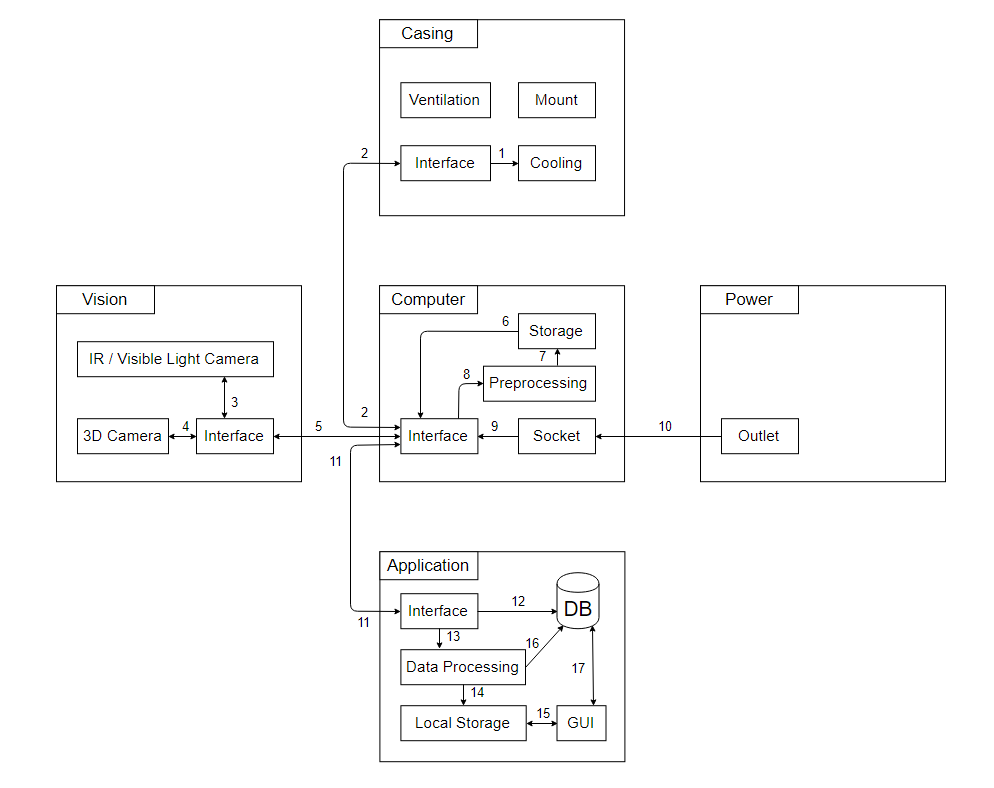
\includegraphics[width=\textwidth]{images/ADS.png}
 \caption{A simple data flow diagram}
\end{figure}

\newpage
\section{Computer Layer Subsystems}
The brain of the Traffic Pi device. Center of the architectural design that sens and receives from the other component layers. Takes in the data acquired from vision, housed in the case, driven from the power layer, and communicates with the application to transmit the desired information for the user. The computer layer determines when to active and record its surroundings and process the data then stores it for further use from the application layer.

\subsection{Interface}
The central bus mechanism the connects to computer layer's surrounding layers.

\begin{figure}[h!]
	\centering
 	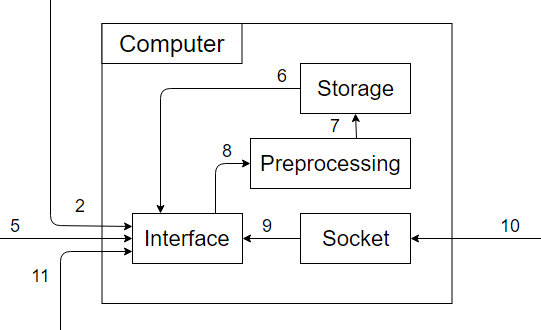
\includegraphics[width=0.60\textwidth]{images/computer_subsystem.png}
 \caption{Computer Interface subsystem diagram}
\end{figure}

\subsubsection{Assumptions}
Assume the interface is uninterrupted and successfully communicates with the other layers and power socket.

\subsubsection{Responsibilities}
Serves as the central hub for transmitting and receiving information from the vision, case, application layers and the power socket sub-layer. Electrical power from the socket will the cooling mechanism and the cameras, then from data collected from vision if a car is detected the computer interface will signal pre-process to take in data like footage (frames), distance, time stamps, and car ID assignment. Will transmit data to the case layer's cooling system to maintain proper temperate condition to avoid overheating given heat generated and environmental heat. Computer interface will once connected to a home computer and commanded to direct stored data for the user it will direct to the application layer's interface. Signals can be redirected back in case of malfunctions, errors, or corrupted data.

\subsubsection{Subsystem Interfaces}

\begin {table}[H]
\caption {Computer interfaces} 
\begin{center}
    \begin{tabular}{ | p{1cm} | p{6cm} | p{3cm} | p{3cm} |}
    \hline
    ID & Description & Inputs & Outputs \\ \hline
    \#2 & Directs power to cooling system and receive temperature data & \pbox{3cm}{Temp data} & \pbox{3cm}{Electric power (watts)}  \\ \hline
    \#5 & Directs power and receive camera data & \pbox{3cm}{Footage (frames) \\ Distance (meters) \\ Car ID} & \pbox{3cm}{Electric power (watts)}  \\ \hline
    \#6 & Storage data stream through Interface and towards the application layer or to continue with normal operations & \pbox{3cm}{N/A} & \pbox{3cm}{Footage (frames) \\ Distance (meters) \\ Car ID \\ Time stamp}  \\ \hline
    \#8 & Data from vision to go through pre-processing to be looked over and formatted for later use or called by user to be displayed on their local machine & \pbox{3cm}{N/A} & \pbox{3cm}{Footage (frames) \\ Distance (meters) \\ Car ID}  \\ \hline
    \#9 & Mechanical socket transmitting electrical power & \pbox{3cm}{Electric power (watts)} & \pbox{3cm}{N/A}  \\ \hline
    \#11 & The Traffic Pi connected with the user's home computer and communicates through the pre-installed program on their machine & \pbox{3cm}{Error Signal} & \pbox{3cm}{Footage (frames) \\ Distance (meters) \\ Car ID \\ Time stamp}  \\ \hline
    \end{tabular}
\end{center}
\end{table}

\subsection{Pre-process}
Takes in the data given from the interface layer and sets up the data format to be stored and later use in the application layer.

\begin{figure}[h!]
	\centering
 	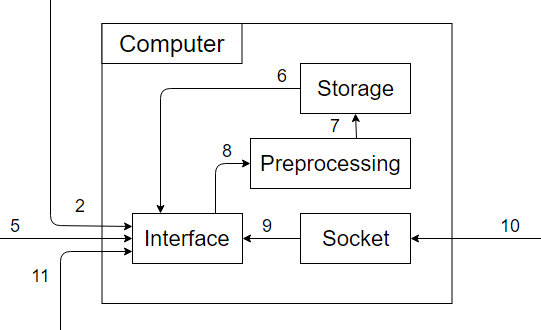
\includegraphics[width=0.60\textwidth]{images/computer_subsystem.png}
 \caption{Pre-process subsystem diagram}
\end{figure}

\subsubsection{Assumptions}
Assume the data collected and given is not corrupted nor illegal for the formatting.

\subsubsection{Responsibilities}
The pre-process sub-layer is responsible for formatting given data from the interface sub-layer from the vision layer. Data given would include footage (frames), distance, time stamps, and car ID assignment, then formats them to be stored in the storage for later processing in the application layer. The purpose of this is to not strain the computer layer's ability to capture the required variable data from passing cars by computing speed and streaming video data at the same time.

\subsubsection{Subsystem Interfaces}

\begin {table}[H]
\caption {Pre-process subsystem interfaces} 
\begin{center}
    \begin{tabular}{ | p{1cm} | p{6cm} | p{3cm} | p{3cm} |}
    \hline
    ID & Description & Inputs & Outputs \\ \hline
    \#7 & Post pre-processing to be stored or signalled by user to collect storage data & \pbox{3cm}{N/A} & \pbox{3cm}{Footage (frames) \\ Distance (meters) \\ Car ID \\ Time stamp}  \\ \hline
    \#8 & Data from vision to go through pre-processing to be looked over and formatted for later use or called by user to be displayed on their local machine & \pbox{3cm}{Footage (frames) \\ Distance (meters) \\ Car ID} & \pbox{3cm}{N/A}  \\ \hline
    \end{tabular}
\end{center}
\end{table}

\subsection{Storage}
The sub-layer tasked to simple store the data from pre-process and later access for future computational work.

\begin{figure}[h!]
	\centering
 	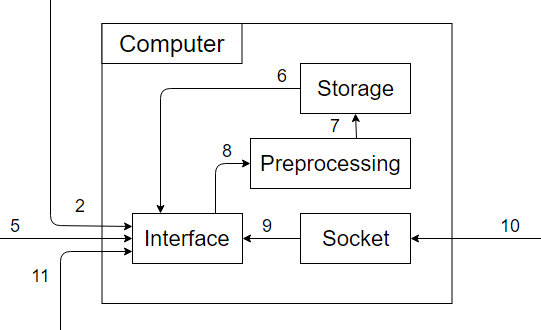
\includegraphics[width=0.60\textwidth]{images/computer_subsystem.png}
 \caption{Storage subsystem diagram}
\end{figure}

\subsubsection{Assumptions}
Assume the storage will be able to hold enough data for a mildly used road and will not fall under mechanical malfunctions.

\subsubsection{Responsibilities}
Storage is to hold formatted files from pre-process and returns the Traffic Pi to continue collecting data. Once the Traffic Pi is picked up and connected to the user's home computer then requested to take the formatted data to be calculated and viewed, the storage sub-system will send the data through computer layer's interface then onto the application layer. If the data was found to be corrupted the  application will request either a troubleshoot or another request of storage's data.

\subsubsection{Subsystem Interfaces}

\begin {table}[H]
\caption {Storage subsystem interfaces} 
\begin{center}
    \begin{tabular}{ | p{1cm} | p{6cm} | p{3cm} | p{3cm} |}
    \hline
    ID & Description & Inputs & Outputs \\ \hline
    \#6 & Continues devices normal operations unless signalled by the user to stream data into their local machine & \pbox{3cm}{Footage (frames) \\ Distance (meters) \\ Car ID \\ Time stamp} & \pbox{3cm}{N/A}  \\ \hline
    \#7 & Post pre-processing to be stored or signalled by user to collect storage data & \pbox{3cm}{Footage (frames) \\ Distance (meters) \\ Car ID \\ Time stamp} & \pbox{3cm}{N/A}  \\ \hline
    \end{tabular}
\end{center}
\end{table}

\subsection{Socket}
A simple mechanical port that transfers electrical power to the Traffic Pi that is given from the power layer.

\begin{figure}[h!]
	\centering
 	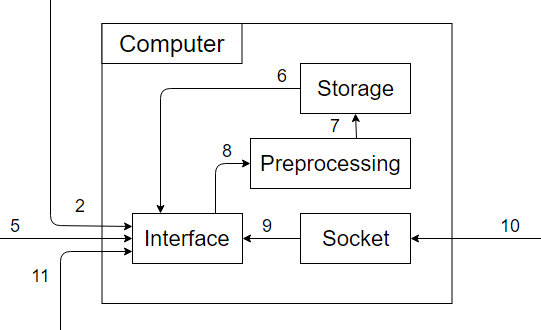
\includegraphics[width=0.60\textwidth]{images/computer_subsystem.png}
 \caption{Socket subsystem diagram}
\end{figure}

\subsubsection{Assumptions}
Assume the electrical socket will not malfunction and correctly sends the desired electrical power for the Traffic Pi to correctly work.

\subsubsection{Responsibilities}
The socket sub-layer will transfer the desired electrical power to the computer layer's interface and to maintain a steady electrical flow of power so the Traffic Pi can continue to function. The socket is depended on correctly receiving the required power from the power layer.

\subsubsection{Subsystem Interfaces}

\begin {table}[H]
\caption {Socket subsystem interfaces} 
\begin{center}
    \begin{tabular}{ | p{1cm} | p{6cm} | p{3cm} | p{3cm} |}
    \hline
    ID & Description & Inputs & Outputs \\ \hline
    \#9 & Mechanical socket transmitting electrical power & \pbox{3cm}{N/A} & \pbox{3cm}{Electric power (watts)}  \\ \hline
    \#10 & The physical implementation of an electric flow of power that allows the device to function & \pbox{3cm}{Electric power (watts)} & \pbox{3cm}{N/A}  \\ \hline
    \end{tabular}
\end{center}
\end{table}


\newpage
\section{Vision Layer Subsystems}
The vision layer controls all of the input from what our project sees. Our current design contains two cameras, one infrared / visible camera and one 3D camera. These two devices will be connected to the main computer (Raspberry Pi) via an interface. While this may not be the best configuration, it allows us to use the IR/Visible camera for detection and the 3D camera to determine the distance between the camera and the vehicle. This is currently the method that we think would work best for capturing the speed of the vehicle. We will also be considering any final methods for capturing the speed before purchasing the 3D camera and implementing it into the system. 

\subsection{Infrared / Visible Light Camera}
This subsystem is for finding each car in sight of the camera. Because it is an infrared and a visible light camera, it will be able to see the street even when cars are driving by. Inside the camera itself are two filters, one for visible light and one for infrared light. These two filters are controlled automatically by the camera and can automatically switch when it is no longer bright enough to see any vehicles. From this camera is a connection to the Vision interface so that if another part of the system needs access to the camera, it can get access through that interface.

\begin{figure}[h!]
	\centering
 	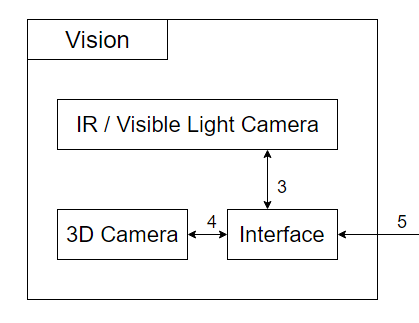
\includegraphics[width=0.60\textwidth]{images/vision_subsystem.png}
 \caption{IR / Visible light subsystem diagram}
\end{figure}

\subsubsection{Assumptions}
We are assuming that the cameras would be able to pick up the cars accurately enough to determine their location on screen. 

\subsubsection{Responsibilities}
The responsibility of the IR / Visible light camera is to be able to see what is in front of it regardless of the amount of light available.

\subsubsection{Subsystem Interfaces}

\begin {table}[H]
\caption {IR / Visible light subsystem interfaces} 
\begin{center}
    \begin{tabular}{ | p{1cm} | p{6cm} | p{3cm} | p{3cm} |}
    \hline
    ID & Description & Inputs & Outputs \\ \hline
    \#1 & Provide video feed from the IR / visible light camera to the interface & \pbox{3cm}{N/A} & \pbox{3cm}{Interface}  \\ \hline
    \end{tabular}
\end{center}
\end{table}

\subsection{3D Camera}
This subsystem is for finding the distance from the camera to any point on the screen. This will be helpful in providing the distance between two points on the frame so that we can more accurately find the distance the vehicle travels. From this camera is a connection to the Vision interface so that if another part of the system needs access to the camera, it can get access through that interface.

\begin{figure}[h!]
	\centering
 	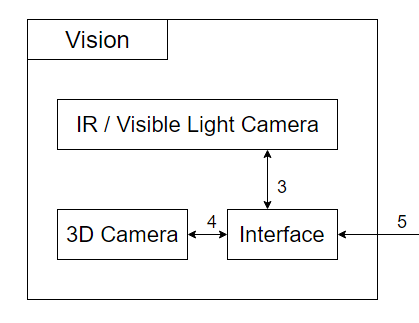
\includegraphics[width=0.60\textwidth]{images/vision_subsystem.png}
 \caption{3D camera subsystem diagram}
\end{figure}

\subsubsection{Assumptions}
We are assuming that the cameras would be able to pick up the cars accurately enough to determine their distance to the camera. 

\subsubsection{Responsibilities}
The responsibility of the 3D camera is to be able to calculate the distance from a point on the frame to the camera. We are also assuming that the camera will be able calculate the distance to the camera and thus the distance between two points on the screen.

\subsubsection{Subsystem Interfaces}

\begin {table}[H]
\caption {3D camera subsystem interfaces} 
\begin{center}
    \begin{tabular}{ | p{1cm} | p{6cm} | p{3cm} | p{3cm} |}
    \hline
    ID & Description & Inputs & Outputs \\ \hline
    \#2 & Provide video feed from the 3D camera to the interface & \pbox{3cm}{N/A} & \pbox{3cm}{Interface}  \\ \hline
    \end{tabular}
\end{center}
\end{table}

\subsection{Vision Interface}
This subsystem is for communicating camera frames outside of the vision system.

\begin{figure}[h!]
	\centering
 	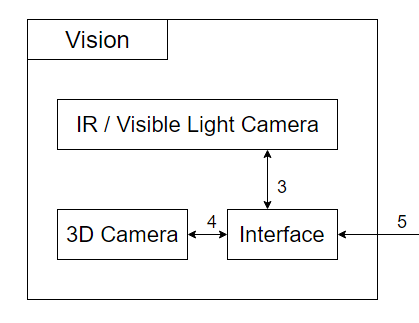
\includegraphics[width=0.60\textwidth]{images/vision_subsystem.png}
 \caption{Vision interface subsystem diagram}
\end{figure}

\subsubsection{Assumptions}
N/A

\subsubsection{Responsibilities}
Transfer information from the cameras to any other system that needs to use it.

\subsubsection{Subsystem Interfaces}

\begin {table}[H]
\caption {Vision interface subsystem interfaces} 
\begin{center}
    \begin{tabular}{ | p{1cm} | p{6cm} | p{3cm} | p{3cm} |}
    \hline
    ID & Description & Inputs & Outputs \\ \hline
    \#3 & Transfer Camera information outside of the vision system & \pbox{3cm}{3D camera, IR/visible light camera, Computer Interface} & \pbox{3cm}{Computer Interface}  \\ \hline
    \end{tabular}
\end{center}
\end{table}

\newpage
\section{Application Layer Subsystems}
We had two possible implementations for the application layer. Had we chosen to do the processing in the cloud, the application layer would have just been a web interface for the user to interact with the system.

\subsection{Interface Subsystem}
The application layer handles communication with the rest of the system. More specifically, the Computer layer. Internally, it communicates with the data processing module and it receives information from the GUI as well.

\begin{figure}[h!]
	\centering
 	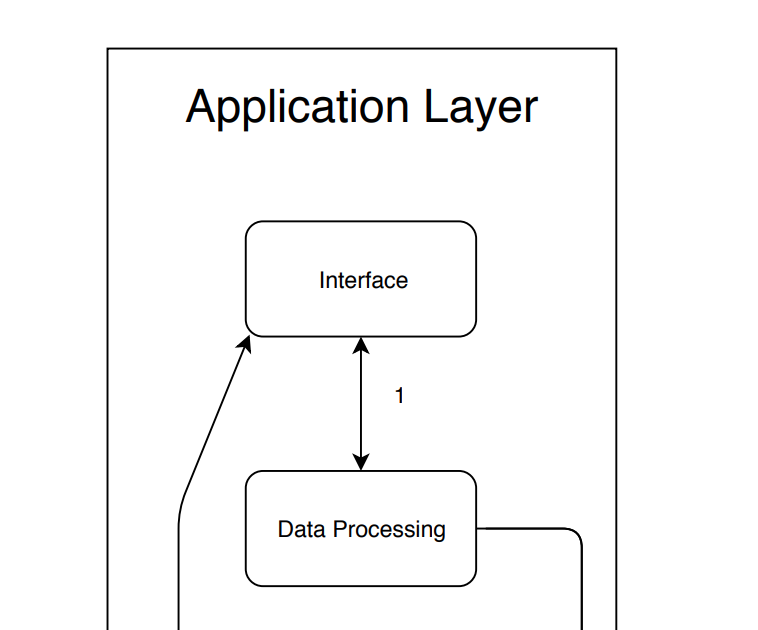
\includegraphics[width=0.60\textwidth]{images/app_sub_1}
 \caption{Interface Subsystem Diagram}
\end{figure}

\subsubsection{Assumptions}
It will receive data from the Computer layer.

\subsubsection{Responsibilities}
As previously stated, the application layer main interface handles communication from the Computer layer. It takes as input raw video from the computer layer and it passes it on to the data processing module. The main interface is synonymous with the graphical user interface which is just the visual representation of data for our system with an added layer of abstraction.

\subsubsection{Subsystem Interfaces}

\begin {table}[H]
\caption {App interface subsystem interfaces} 
\begin{center}
    \begin{tabular}{ | p{1cm} | p{6cm} | p{3cm} | p{3cm} |}
    \hline
    ID & Description & Inputs & Outputs \\ \hline
    \#0 & Handles communication between the application layer and the rest of the system & \pbox{3cm}{warning messages \\ Data} & \pbox{3cm}{Pre-processed video}  \\ \hline
    \end{tabular}
\end{center}
\end{table}


\subsection{Data Processing Subsystem}
This modules simply takes video as input and outputs an analyzed/condensed version of the input.

\begin{figure}[h!]
	\centering
 	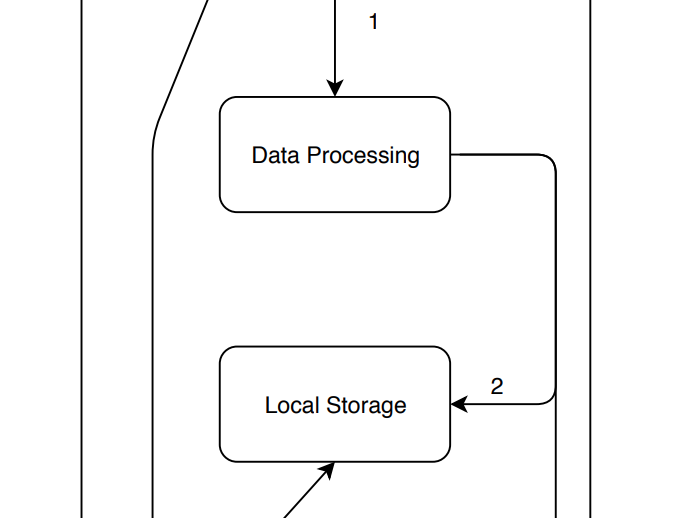
\includegraphics[width=0.60\textwidth]{images/app_sub_2_1}
 \caption{Data processing subsystem Diagram}
\end{figure}

\subsubsection{Assumptions}
The Computer layer completed the pre-processing successfully.

\subsubsection{Responsibilities}
This subsystem handle putting the bounding boxes around every vehicle along with measuring and recording the speed of every vehicle that the system deems to be appropriate. The data processing module also filters out anything that is not a vehicle.

\subsubsection{Subsystem Interfaces}

\begin {table}[H]
\caption {Data processing subsystem interfaces} 
\begin{center}
    \begin{tabular}{ | p{1cm} | p{6cm} | p{3cm} | p{3cm} |}
    \hline
    ID & Description & Inputs & Outputs \\ \hline
    \#1 & Handles the video processing & \pbox{3cm}{pre-processed video} & \pbox{3cm}{processed video \\ Analytics}  \\ \hline
    \end{tabular}
\end{center}
\end{table}

\subsection{Local Storage Subsystem}
Archives the analyzed video from the data processing module.

\begin{figure}[h!]
	\centering
 	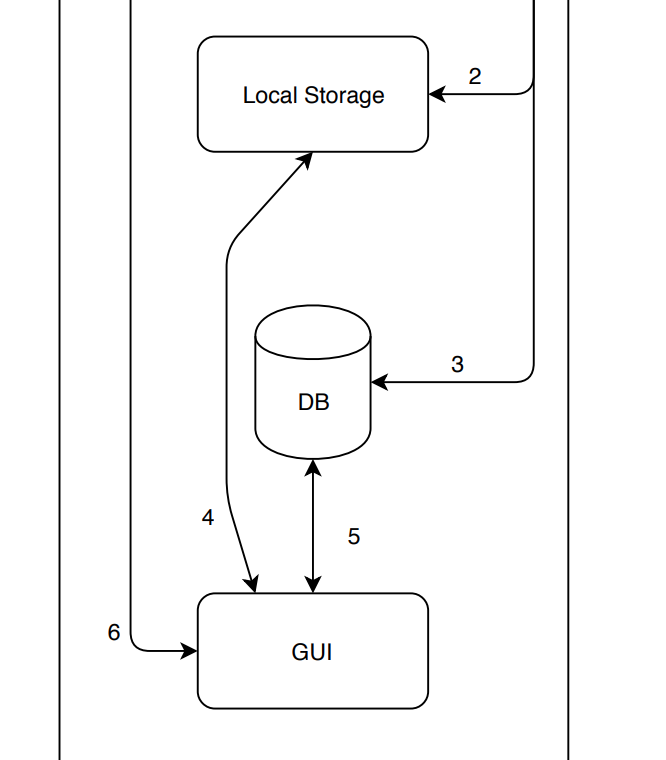
\includegraphics[width=0.60\textwidth]{images/app_sub_3}
 \caption{Local Storage subsystem Diagram}
\end{figure}

\subsubsection{Assumptions}
There will be sufficient local storage available.

\subsubsection{Responsibilities}
Simply archives the analyzed video from the data processing module so that the user has access to it from the GUI.

\subsubsection{Subsystem Interfaces}

\begin {table}[H]
\caption {Local Storage subsystem interfaces} 
\begin{center}
    \begin{tabular}{ | p{1cm} | p{6cm} | p{3cm} | p{3cm} |}
    \hline
    ID & Description & Inputs & Outputs \\ \hline
    \#2 & Archives analyzed video & \pbox{3cm}{Processed video \\ error messages} & \pbox{3cm}{processed videos}  \\ \hline
    \end{tabular}
\end{center}
\end{table}

\subsection{Database Subsystem}
A local database that archives analytics from the traffic study that is being conducted.

\begin{figure}[h!]
	\centering
 	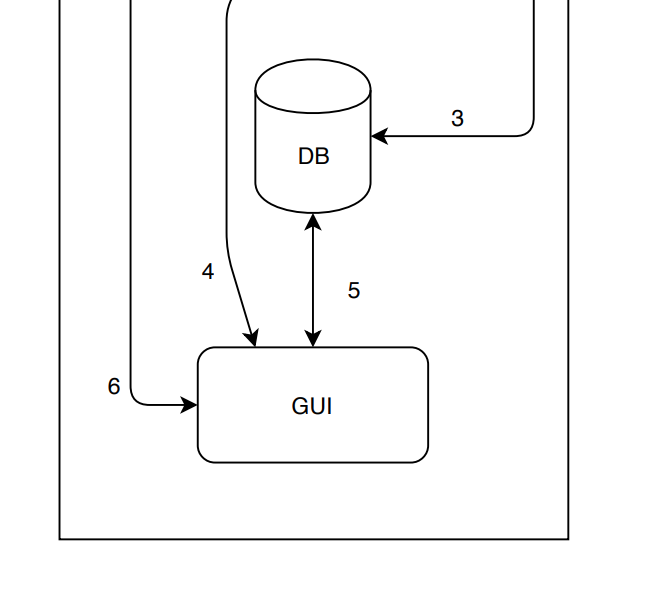
\includegraphics[width=0.60\textwidth]{images/app_sub_4}
 \caption{Database subsystem Diagram}
\end{figure}

\subsubsection{Assumptions}
It can be hosted on the local machine.

\subsubsection{Responsibilities}
The database takes data in from the data processing module. The GUI will be able to pull information from the database.

\subsubsection{Subsystem Interfaces}

\begin {table}[H]
\caption {Database subsystem interfaces} 
\begin{center}
    \begin{tabular}{ | p{1cm} | p{6cm} | p{3cm} | p{3cm} |}
    \hline
    ID & Description & Inputs & Outputs \\ \hline
    \#3 & Archives data from the traffic study & \pbox{3cm}{Processed data \\ Action from GUI} & \pbox{3cm}{Data for GUI}  \\ \hline
    \end{tabular}
\end{center}
\end{table}

\subsection{Graphical User Interface Subsystem}
The graphical user interface will allow the user to interact with the system. 

\begin{figure}[h!]
	\centering
 	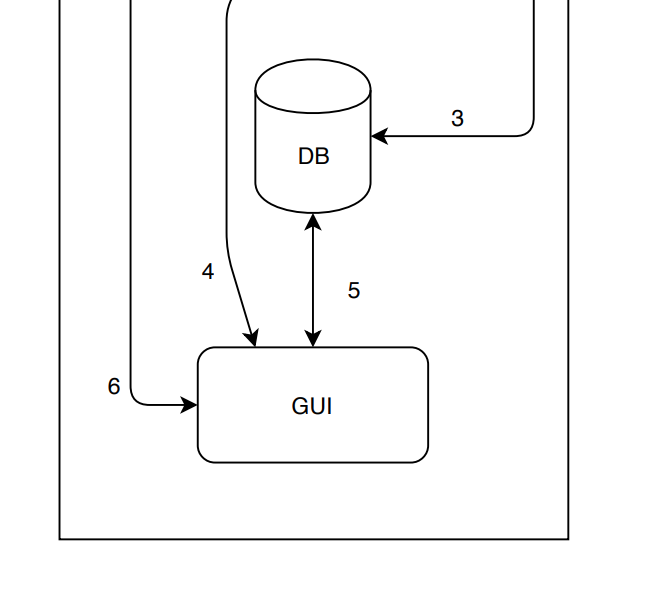
\includegraphics[width=0.60\textwidth]{images/app_sub_4}
 \caption{GUI Subsystem Diagram}
\end{figure}

\subsubsection{Assumptions}
The rest of the application layer functions properly.

\subsubsection{Responsibilities}
The user will be presented with a few options. They will be able to configure a few system options like setting the recording time intervals. They will have the option to be presented with a dashboard that has the visual representations of all the data in the form of graphs and tables. The user will also be able to see the recorded video and to start a new traffic study which deletes old data/video.

\subsubsection{Subsystem Interfaces}

\begin {table}[H]
\caption {Graphical User Interface Subsystem interfaces} 
\begin{center}
    \begin{tabular}{ | p{1cm} | p{6cm} | p{3cm} | p{3cm} |}
    \hline
    ID & Description & Inputs & Outputs \\ \hline
    \#4,5,6 & Allows the user to interact with the system & \pbox{3cm}{Data about system status \\ Current local storage space, videos \\ Data from DB} & \pbox{3cm}{Error messages \\ Data deletion option for both LS and DB}  \\ \hline
    \end{tabular}
\end{center}
\end{table}




\newpage
\section{Case Layer Subsystems}
The case layer is the component that will house the physical components of the Traffic Pi system. This layer is comprised of four subsystems: a mounting plate, cooling, ventilation, and an interface. Each subsystem is responsible in some part for maintaining and protecting the physical components of the Traffic Pi system.

\subsection{Mounting Plate}
The mounting plate is detachable component of the case that can be attached to most camera tripods sold on the market. This subsystem is a part of the Traffic Pi system as a whole to facilitate the attaching of the system of a common item such as a tripod.

\begin{figure}[h!]
	\centering
 	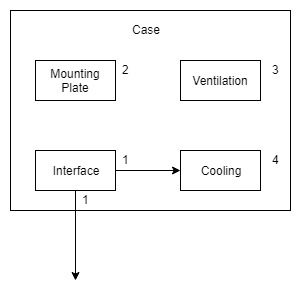
\includegraphics[width=0.60\textwidth]{images/case_layer}
 \caption{Case Layer Subsystem 2: Mounting Plate}
\end{figure}

\subsubsection{Assumptions}
It is assumed that the designed mounting plate included on the case for the Traffic Pi is suitable for mounting on most tripods on sold on the market.

\subsubsection{Responsibilities}
It is the responsibility of the mounting plate to provide the user of the Traffic Pi an easy to use location on the Traffic Pi such that a user may mount it to a standard camera tripod with ease.

\subsubsection{Subsystem Interfaces}
The interface for this subsystem is of a physical nature. The only input being the screw that is a detachable part of the mounting plate.

\begin {table}[H]
\caption {Mounting Plate interfaces} 
\begin{center}
    \begin{tabular}{ | p{1cm} | p{6cm} | p{3cm} | p{3cm} |}
    \hline
    ID & Description & Inputs & Outputs \\ \hline
    01 & Steel Screw 3/8 Inch & \pbox{3cm}{Steel Screw} & \pbox{3cm}{N/A}  \\ \hline
    \end{tabular}
\end{center}
\end{table}

\subsection{Cooling}
The cooling subsystem in the case layer is a component meant to keep the system within safe operating temperatures. This component draws power from the Raspberry Pi and operates whenever the Traffic Pi system is in use. 

\begin{figure}[h!]
	\centering
 	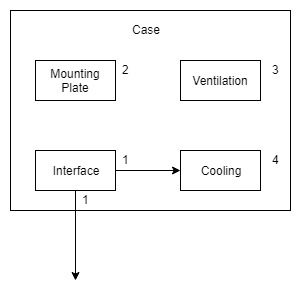
\includegraphics[width=0.60\textwidth]{images/case_layer}
 \caption{Case Layer Subsystem 4: Cooling}
\end{figure}

\subsubsection{Assumptions}
It is assumed that the cooling component of the case is able to draw sufficient power from the Raspberry Pi to operate efficiently. Further it is assumed that continued use of the cooling component will impact performance of the Traffic Pi system.

\subsubsection{Responsibilities}
It is the responsibility of the cooling subsystem to keep the Raspberry Pi, IR camera, and 3D camera in a temperature range that rated for these devices, -30 C to 80 C.

\subsubsection{Subsystem Interfaces}
The interface for this subsystem is of a physical nature. The only input being the screw that is a detachable part of the mounting plate.

\begin {table}[H]
\caption {Cooling Interfaces} 
\begin{center}
    \begin{tabular}{ | p{1cm} | p{6cm} | p{3cm} | p{3cm} |}
    \hline
    ID & Description & Inputs & Outputs \\ \hline
    04 & Power from the Raspberry Pi & \pbox{3cm}{Interface} & \pbox{3cm}{N/A}  \\ \hline
    \end{tabular}
\end{center}
\end{table}

\subsection{Ventilation}
The ventilation component of the case layer is intended to allow any heat generated by use of the Traffic Pi system to dissipate in a controlled manner. The Raspberry Pi in particular will generate heat upon use of the system and although a cooling component is available, this ventilation subsystem will allow further dissipation of heat.

\begin{figure}[h!]
	\centering
 	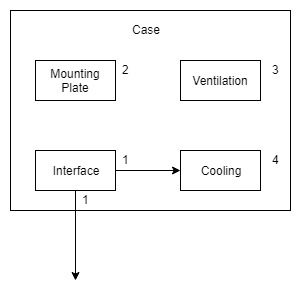
\includegraphics[width=0.60\textwidth]{images/case_layer}
 \caption{Case Layer Subsystem 3: Ventilation}
\end{figure}

\subsubsection{Assumptions}
It is assumed that this ventilation subsystem in conjunction with the cooling subsystem is sufficient enough to keep the system within safe operating temperatures.

\subsubsection{Responsibilities}
It is the responsibility of the ventilation subsystem to allow heat generated from the Raspberry Pi, IR camera, and 3D camera to safely dissipate away from the system.

\subsubsection{Subsystem Interfaces}
This component does not interact with any other subsystem.

\subsection{Interface}
The interface subsystem in the case layer is a component meant to provide power to the cooling subsystem which has been directed from the Traffic Pi. This interface is purely hardware in nature, a standard USB Type C cable. 

\begin{figure}[h!]
	\centering
 	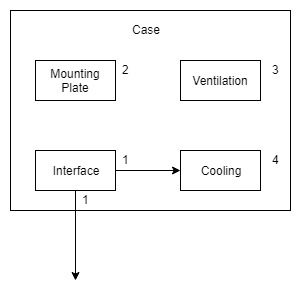
\includegraphics[width=0.60\textwidth]{images/case_layer}
 \caption{Case Layer Subsystem 1: Interface}
\end{figure}

\subsubsection{Assumptions}
It is assumed that the interface cable is able to transmit the necessary power requirements of the cooling subsystem from the Raspberry Pi.

\subsubsection{Responsibilities}
It is the responsibility of the interface to provide a conduit of power from the Raspberry Pi to the cooling subsystem.

\subsubsection{Subsystem Interfaces}
This subsystem interfaces with the Raspberry Pi and Cooling subsystems.

\begin {table}[H]
\caption {Interfaces} 
\begin{center}
    \begin{tabular}{ | p{1cm} | p{6cm} | p{3cm} | p{3cm} |}
    \hline
    ID & Description & Inputs & Outputs \\ \hline
    04 & USB Type C Cable & \pbox{3cm}{Power from Raspberry Pi} & \pbox{3cm}{Power to Cooling}  \\ \hline
    \end{tabular}
\end{center}
\end{table}
\newpage
\section{Power Layer Subsystems}
The power subsystem is the as the name suggests the subsystem handling power for the Traffic Pi. Rather than pursuing a mobile power source of which size, duration of power, reliability, maintenance, and other characteristics play a part, the standard AC power cable that comes with a Raspberry Pi will be used to provide power to the entire system. 

\subsection{Power Cable}
The singular subsystem for the Power layer is the power cable for the Raspberry Pi. A power cable for connection to an AC wall outlet (5.1V micro USB supply) comes standard with most Raspberry Pi's. This subsystem will provide power to the Raspbery Pi which serves as the main computer "brain" for the Traffic Pi system.

\begin{figure}[h!]
	\centering
 	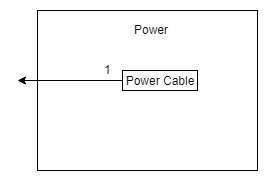
\includegraphics[width=0.60\textwidth]{images/power_layer}
 \caption{Power Layer}
\end{figure}

\subsubsection{Assumptions}
It is assumed that the 5.1V micro USB supply cable, when plugged into a standard US AC wall outlet will be able to supply sufficient Voltage to the Traffic Pi system (the Raspberry Pi, 3D camera, and IR camera) without strain or stress on either the system or power source.

\subsubsection{Responsibilities}
The power cable subsystem is responsible for providing sustained, constant, steady power for the Raspberry Pi that is part of the Traffic Pi system as a whole. 

\subsubsection{Subsystem Interfaces}
The power layer is unique in that it does not require a strict "interface" subsystem for communicating with the other layers in the Traffic Pi system. The power cable subsystem directly interfaces with the USB power supply socket on the Raspberry Pi.

\begin {table}[H]
\caption {Power cable subsystem interfaces} 
\begin{center}
    \begin{tabular}{ | p{1cm} | p{6cm} | p{3cm} | p{3cm} |}
    \hline
    ID & Description & Inputs & Outputs \\ \hline
    01 & 5.1V micro USB supply & \pbox{3cm}{N/A} & \pbox{3cm}{1 Amp}  \\ \hline
    \end{tabular}
\end{center}
\end{table}
\newpage

%%% References
\bibliographystyle{plain}
\bibliographystyle{reference/IEEEtran_custom}
\bibliography{reference/refs}{}

\end{document}